\documentclass[tikz]{standalone}
\usepackage{pgfplots}
\pgfplotsset{compat=1.15}
\usepackage{mathrsfs}
\usetikzlibrary{arrows,calc}
\usepackage{tkz-euclide}
\pagestyle{empty}

\definecolor{AngleClr}{rgb}{0,0.39215686274509803,0}
\definecolor{ShapeClr}{rgb}{0.6,0.2,0}

\begin{document}

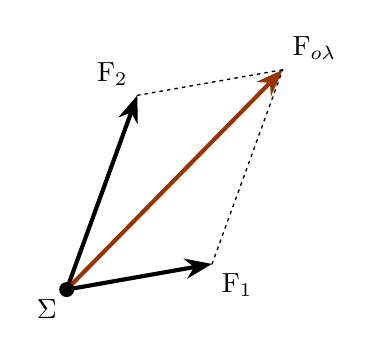
\begin{tikzpicture}[scale=.75]
\tkzSetUpLine[line width=1pt,color=black]
\tkzSetUpPoint[fill=black]

\tkzDefPoint(0,0){B}
\tkzDefPoint(70:3.5){A}
\tkzDefShiftPointCoord[B](10:2.5){C}
\tkzDefShiftPointCoord[A](10:2.5){D}

\tkzDrawSegments[line width=1.5pt,-Stealth,color=black](B,A B,C)
\tkzDrawSegments[line width=1.5pt,-Stealth,color=ShapeClr](B,D)
\tkzDrawSegments[line width=0.5pt,color=black,dashed,dash pattern=on 1pt off 1.75pt](A,D C,D)

\tkzDrawPoints[size=5](B)
\tkzLabelPoint[above left](A){${\rm F}_2$}
\tkzLabelPoint[below left](B){$\rm \Sigma$}
\tkzLabelPoint[below right](C){${\rm F}_1$};
\tkzLabelPoint[above right](D){${\rm F}_{o\lambda}$};


\end{tikzpicture}

\end{document}
